\documentclass[../main.tex]{subfiles}

\usepackage{nopageno} %Seitenzahlen auf richtiger Seite 

\usepackage[left=2cm, right=2cm, top=2cm, includehead, includefoot, headheight=17pt]{geometry}

\usepackage[utf8x]{inputenc}
\usepackage[english]{babel}
\usepackage{amsmath,amssymb,amsthm}
\usepackage{framed}
\usepackage{wasysym}
\usepackage[T1]{fontenc} %Silbentrennung 
\usepackage{color} %Farbe
\usepackage{graphicx}
\usepackage{float}%Grafik am gleichen Ort plazieren
%pdf. png. einfach eingliedern
\usepackage{subfigure} %Grafiken nebeneinander
\usepackage{pdfpages}
\usepackage{ulem} 	%\uuline{urgent}    % doppelt unterstreichen
%\uwave{boat}      % unterschlängeln
%\sout{wrong}       % durchstreichen
%\xout{removed}     % ausstreichen mit //////.

\usepackage{tikz}
\usetikzlibrary{trees}
\usetikzlibrary{plotmarks}
\usetikzlibrary{angles,quotes,babel}
\usetikzlibrary{shadings}
\usetikzlibrary{patterns}
\usetikzlibrary{matrix}
\usetikzlibrary{arrows}
\usetikzlibrary{calc}

\usepackage{pgfplots}
\usepackage{pgf-pie}
\pgfplotsset{compat=1.10}
\usepgfplotslibrary{statistics}
\usepgfplotslibrary{fillbetween}

\usepackage{tkz-euclide}
\usepackage{enumerate}
\usepackage{stmaryrd}
\usepackage{tabularx}
\usepackage{wrapfig}
\usepackage{epsdice}
\usepackage{multirow}
\usepackage{rotating}
\usepackage{pdflscape}
\usepackage{fancyhdr}

\pagestyle{fancy} %eigener Seitenstil
\fancyhf{} %alle Kopf- und Fußzeilenfelder bereinigen
\fancyhead[L]{} %Kopfzeile links
\fancyhead[C]{} %zentrierte Kopfzeile
\fancyhead[R]{} %Kopfzeile rechts
\renewcommand{\headrulewidth}{0.4pt} %obere Trennlinie
\fancyfoot[C]{\thepage} %Seitennummer
\renewcommand{\footrulewidth}{0.4pt} %untere Trennlinie

% Number spaces 
\newcommand{\CC}{\ensuremath{\mathbb{C}}}
\newcommand{\RR}{\ensuremath{\mathbb{R}}}
\newcommand{\QQ}{\ensuremath{\mathbb{Q}}}
\newcommand{\ZZ}{\ensuremath{\mathbb{Z}}}
\newcommand{\NN}{\ensuremath{\mathbb{N}}}
\newcommand{\LL}{\ensuremath{\mathbb{L}}}
\newcommand{\DD}{\ensuremath{\mathbb{D}}}
\newcommand{\WW}{\ensuremath{\mathbb{W}}}

%draw chemestry molecules 
\usepackage{chemfig} % https://mirror.ox.ac.uk/sites/ctan.org/macros/generic/chemfig/

\newcommand\vv[1]{%
	\begin{tikzpicture}[baseline=(arg.base)]
		\node[inner xsep=0pt] (arg) {$#1$};
		\draw[line cap=round,line width=0.45,->,shorten >= 0.2pt, shorten <= 0.7pt] (arg.north west) -- (arg.north east);
	\end{tikzpicture}%
} %command will render \vv{x} with an arrow aboth 

\renewcommand{\labelenumi}{\roman{enumi})}

\DeclareMathOperator{\ggT}{ggT}
\DeclareMathOperator{\sign}{sign}

%sections
\theoremstyle{plain}
\newtheorem{Thm}{Theorem}[section]
\newtheorem{Def}[Thm]{Definition}
\newtheorem{Prop}[Thm]{Proposition}

\theoremstyle{definition}
\newtheorem{lemma}[Thm]{Lemma}
\newtheorem{corollary}[Thm]{Corollary}
\newtheorem{claim}[Thm]{Claim}
\newtheorem{Proof}[Thm]{Proof}
\newtheorem{Ex}[Thm]{Example}

\newtheorem{Exercise}{ex}[section] %follow proper enum
\newtheorem{ex}[Exercise]{Exercise}
\newtheorem{Solution}{sol}[section]
\newtheorem{sol}[Solution]{Solution}

\theoremstyle{remark}
\newtheorem{remark}[Thm]{Remark} % follows thm enum

\newtheorem{comment}{Comment}[section] %follow comment enum
\newtheorem{notation}[comment]{Notation}
\newtheorem{reasoning}[comment]{Reasoning}
\newtheorem{Intpr}[comment]{Interpretation}

%some premmade with title (uterwise use \textbf{Title} ...)
\newenvironment{ThmWithTitle}[1]{%
	\begin{Thm}[\textbf{#1}]}{\end{Thm}}
\newenvironment{PropWithTitle}[1]{%
	\begin{Prop}[\textbf{#1}]}{\end{Prop}}
\newenvironment{ExWithTitle}[1]{%
	\begin{Ex}[\textbf{#1}]}{\end{Ex}}
\newenvironment{DefWithTitle}[1]{%
	\begin{Def}[\textbf{#1}]}{\end{Def}}
\newenvironment{RemarkWithTitel}[1]{%
	\begin{remark}[\textbf{#1}]}{\end{remark}}

%format of paragraph 
\renewcommand\paragraph{\@startsection{paragraph}{4}{\z@}%
	{-2.5ex\@plus -1ex \@minus -.25ex}%
	{1.25ex \@plus .25ex}%
	{\normalfont\normalsize\bfseries}}
\makeatother
\setcounter{secnumdepth}{4} % how many sectioning levels to assign numbers to
\setcounter{tocdepth}{4}    % how many sectioning levels to show in ToC

\newcounter{row} 
\renewcommand\therow{\alph{row}} %hier a,b,c etc. def und mit therow abrufbar

\newenvironment{aufz}
{\setcounter{row}{0}%
	\par\noindent\tabularx{\linewidth}[t]
	{\cdot{20}{>{\stepcounter{row}\makebox[1.5em][l]{\therow)\hfill}}X}} %bis max 20 Elemente nebeinander
}
{\endtabularx}


%biblio
\usepackage[]{biblatex}
\addbibresource{referenzenma.bib} 

%glossary
\usepackage{glossaries}
\usepackage{import}


\usepackage{rotating} % Include this package in the preamble

\newglossaryentry{BP230}{
	name={BP230},
	description={A hemidesmosomal protein that connects plectin and keratin filaments to integrins in epithelial cells.}
}

\newglossaryentry{Ca2}{
	name={Ca2+},
	description={Calcium ions essential for cadherin-mediated adhesion by stabilizing cadherin domains and preventing molecular flexibility.}
}

\newglossaryentry{Collagenfibrils}{
	name={Collagen fibrils},
	description={Bundles of collagen molecules aligned in a staggered fashion, forming the structural framework of connective tissues.}
}

\newglossaryentry{EGFepidermalgrowthfactor}{
	name={EGF},
	description={A cell biology concept related to EGF (epidermal growth factor), requiring further specification.}
}

\newglossaryentry{integrin}{
	name={Integrin},
	description={A family of transmembrane receptors that mediate cell adhesion to the extracellular matrix and other cells. They link the cytoskeleton to the ECM and transmit bidirectional signals to regulate cell shape, motility, and survival.}
}

\newglossaryentry{EMT}{
	name={EMT},
	description={Epithelial-to-mesenchymal transition, a process where epithelial cells lose adhesion and gain migratory, invasive properties.}
}

\newglossaryentry{FN1}{
	name={FN1},
	description={One of the repeating domains in fibronectin responsible for collagen and fibrin binding.}
}

\newglossaryentry{FN2}{
	name={FN2},
	description={A fibronectin domain that contributes to binding interactions within the ECM.}
}

\newglossaryentry{FN3}{
	name={FN3},
	description={A fibronectin domain that contains the RGD motif for integrin binding, crucial for cell adhesion.}
}

\newglossaryentry{useless}{
	name={GPCR},
	description={G-protein-coupled receptor; activates intracellular signaling cascades including those that lead to integrin activation.}
}

\newglossaryentry{GTPase}{
	name={GTPase},
	description={A family of enzymes that hydrolyze GTP and regulate many signaling pathways, including cell adhesion and migration.}
}

\newglossaryentry{GTPaseRac}{
	name={GTPase Rac},
	description={A small GTPase that promotes actin polymerization and junction expansion during early cell-cell adhesion.}
}

\newglossaryentry{GTPaseRho}{
	name={GTPase Rho},
	description={A GTPase that promotes actomyosin contractility and maturation of adherens junctions into linear actin bundles.}
}

\newglossaryentry{Gapjunctions}{
	name={Gap junctions},
	description={Specialized intercellular connections composed of connexons that allow direct cytoplasmic exchange of small molecules and ions between neighboring cells.}
}

\newglossaryentry{Golgiapparatus}{
	name={Golgi apparatus},
	description={A cell organelle where glycosylation and processing of ECM proteins like procollagen occur before secretion.}
}

\newglossaryentry{hydroxylysyl}{
	name={Hydroxylysyl (Hyl)},
	description={A hydroxylated derivative of lysine found in collagen. It plays a critical role in forming covalent cross-links between collagen molecules, enhancing tensile strength of the extracellular matrix.}
}

\newglossaryentry{IGFBPInsulingrowthbindingfactor}{
	name={IGFBP},
	description={Insulin growth binding factor, a protein domain found in ECM components that binds insulin-like growth factors, modulating their availability and activity.}
}

\newglossaryentry{Integrin}{
	name={Integrin},
	description={A family of transmembrane receptors that link ECM proteins to the cytoskeleton and mediate bidirectional signaling.}
}

\newglossaryentry{Laminin}{
	name={Laminin},
	description={A cell biology concept related to Laminin, requiring further specification.}
}

\newglossaryentry{Laminin111}{
	name={Laminin-111},
	description={A trimeric laminin isoform found mainly in embryonic tissues, composed of α1, β1, and γ1 chains, crucial for basement membrane structure.}
}

\newglossaryentry{MET}{
	name={MET},
	description={Mesenchymal-to-epithelial transition, where mesenchymal cells adopt epithelial characteristics and form structured tissues.}
}

\newglossaryentry{Phosphoinositide}{
	name={Phosphoinositide},
	description={A lipid component of the membrane that binds Talin and other proteins to regulate integrin activation.}
}

\newglossaryentry{RIAM}{
	name={RIAM},
	description={An adaptor protein that helps recruit Talin to the plasma membrane during integrin activation.}
}

\newglossaryentry{Rap1}{
	name={Rap1},
	description={A small GTPase involved in inside-out signaling to activate integrins during processes like platelet adhesion.}
}

\newglossaryentry{Slug}{
	name={Slug},
	description={Slug is a transcription factor that regulates EMT by repressing epithelial genes and promoting mesenchymal traits.}
}

\newglossaryentry{Snail}{
	name={Snail},
	description={Snail is a transcription factor that regulates EMT by repressing epithelial genes and promoting mesenchymal traits.}
}

\newglossaryentry{Talin}{
	name={Talin},
	description={A cytoskeletal adaptor protein that connects integrins to actin and unfolds under tension to recruit vinculin.}
}

\newglossaryentry{Twist}{
	name={Twist},
	description={Twist is a transcription factor that regulates EMT by repressing epithelial genes and promoting mesenchymal traits.}
}

\newglossaryentry{VitaminC}{
	name={Vitamin-C},
	description={A cofactor required for the hydroxylation of proline and lysine during collagen synthesis. Its deficiency impairs collagen stability.}
}

\newglossaryentry{Zeb}{
	name={Zeb},
	description={Zeb is a transcription factor that regulates EMT by repressing epithelial genes and promoting mesenchymal traits.}
}

\newglossaryentry{actin}{
	name={actin},
	description={A cytoskeletal protein that forms filaments involved in maintaining cell shape and enabling junction formation and contractility.}
}

\newglossaryentry{actinlinkedjunctions}{
	name={actin-linked junctions},
	description={Also known as actin filament attachment sites, these junctions connect actin filaments to cadherins or integrins, supporting adhesion.}
}

\newglossaryentry{adherensjunctions}{
	name={adherens junctions},
	description={Junctions that connect actin filaments between cells via cadherins and adaptor proteins like β-catenin and α-catenin.}
}

\newglossaryentry{adhesionbelt}{
	name={adhesion belt},
	description={A continuous band of adherens junctions linked to actin filaments, providing mechanical integrity and shaping epithelial sheets.}
}

\newglossaryentry{aggrecan}{
	name={aggrecan},
	description={A large proteoglycan with multiple GAG chains that binds hyaluronan to form large ECM aggregates, especially in cartilage.}
}

\newglossaryentry{alphacatenin}{
	name={alpha catenin},
	description={An adaptor protein connecting cadherin-bound β-catenin to actin filaments, enabling dynamic junction regulation.}
}

\newglossaryentry{anchoringjunctions}{
	name={anchoring junctions},
	description={Junctions that attach cells to each other or to the ECM, including adherens junctions, desmosomes, hemidesmosomes, and actin-linked adhesions.}
}

\newglossaryentry{apicalposition}{
	name={apical position},
	description={Refers to the topmost region of an epithelial cell, facing the lumen or external environment. Tight junctions typically occupy this position.}
}

\newglossaryentry{basallamina}{
	name={basal lamina},
	description={A specialized form of extracellular matrix separating epithelial and connective tissue. Composed of laminin, type IV collagen, nidogen, and perlecan.}
}

\newglossaryentry{betacatenin}{
	name={beta-catenin},
	description={A cytoplasmic adaptor protein linking cadherins to actin and also involved in Wnt signaling when stabilized.}
}

\newglossaryentry{bullouspemphigold}{
	name={bullous pemphigold},
	description={An autoimmune skin disease where antibodies target hemidesmosomal proteins, causing blistering.}
}

\newglossaryentry{cadherin}{
	name={cadherin},
	description={A calcium-dependent adhesion molecule mediating homophilic binding between cells. Crucial in adherens junctions and desmosomes.}
}

\newglossaryentry{cadherindomain}{
	name={cadherin domain},
	description={Repeating extracellular domains of cadherins that bind calcium ions and mediate adhesion via N-terminal interactions.}
}

\newglossaryentry{celljunctions}{
	name={cell junctions},
	description={Structures that link adjacent cells or cells to the ECM. Include anchoring, occluding, channel-forming, and signal-relaying junctions.}
}

\newglossaryentry{channelformingjunctions}{
	name={channel-forming junctions},
	description={Junctions that create pores between adjacent cells, allowing the exchange of ions and small molecules. Gap junctions are the primary example in animal cells.}
}

\newglossaryentry{chaperonins}{
	name={chaperonins},
	description={Proteins that assist in the proper folding of procollagen triple helices during synthesis in the endoplasmic reticulum.}
}

\newglossaryentry{chemicalsynapses}{
	name={chemical synapses},
	description={Junctions in the nervous system where neurotransmitters are released to relay signals between neurons or to target cells.}
}

\newglossaryentry{chondroitinsulfate}{
	name={chondroitin sulfate},
	description={A sulfated GAG composed of repeating disaccharides that provides compressive strength to cartilage and connective tissues.}
}

\newglossaryentry{claudin}{
	name={claudin},
	description={A four-pass transmembrane protein forming the backbone of tight junction strands and regulating paracellular permeability.}
}

\newglossaryentry{collagenI}{
	name={collagen I},
	description={The most abundant collagen type in the body, forming fibrils and fibers in skin, bone, tendons, and other tissues.}
}

\newglossaryentry{collagenXVII}{
	name={collagen XVII},
	description={A transmembrane collagen found in hemidesmosomes, anchoring epithelial cells to the basal lamina.}
}

\newglossaryentry{collagenfibers}{
	name={collagen fibers},
	description={Fibrous components of the ECM providing tensile strength. Composed of tightly packed collagen triple helices forming fibrils and bundles.}
}

\newglossaryentry{connectivetissue}{
	name={connective tissue},
	description={Tissue type that supports and anchors other tissues. It contains extracellular matrix rich in fibers like collagen and is separated from epithelium by the basal lamina.}
}

\newglossaryentry{connexin}{
	name={connexin},
	description={A family of proteins that assemble into connexons, enabling the formation of gap junction channels between cells.}
}

\newglossaryentry{connexon}{
	name={connexon},
	description={A hexameric protein assembly forming half of a gap junction channel, made up of six connexin subunits.}
}

\newglossaryentry{cytoskeletalproteins}{
	name={cytoskeletal proteins},
	description={Proteins like actin and intermediate filaments that provide structural integrity and connect to cell junctions for force transmission.}
}

\newglossaryentry{decorin}{
	name={decorin},
	description={A small proteoglycan with a single GAG chain, known to bind collagen fibrils and regulate ECM assembly.}
}

\newglossaryentry{desmocollins}{
	name={desmocollins},
	description={Nonclassical cadherins that function similarly to desmogleins in forming stable desmosomal junctions.}
}

\newglossaryentry{desmogleins}{
	name={desmogleins},
	description={Nonclassical cadherins found in desmosomes that mediate cell-cell adhesion through intermediate filaments.}
}

\newglossaryentry{desmoplakin}{
	name={desmoplakin},
	description={A key desmosomal protein that anchors intermediate filaments to the desmosomal plaque.}
}

\newglossaryentry{desmosomes}{
	name={desmosomes},
	description={Cell-cell anchoring junctions linking intermediate filaments via nonclassical cadherins such as desmogleins and desmocollins.}
}

\newglossaryentry{dystroglycan}{
	name={dystroglycan},
	description={A transmembrane receptor in muscle and epithelial cells that connects the cytoskeleton to the basal lamina via laminin.}
}

\newglossaryentry{ectoderm}{
	name={ectoderm},
	description={The outermost embryonic germ layer that gives rise to the epidermis, nervous system, and related structures.}
}

\newglossaryentry{elastin}{
	name={elastin},
	description={A protein that forms elastic fibers in the ECM, allowing tissues like lungs and skin to stretch and recoil.}
}

\newglossaryentry{epithelialtissue}{
	name={epithelial tissue},
	description={A tissue type that forms tightly connected cell layers, covering body surfaces and lining cavities. It plays a role in protection, secretion, and selective permeability.}
}

\newglossaryentry{extracellularmatrix}{
	name={extracellular matrix},
	description={A complex network of proteins and polysaccharides outside cells. It includes collagen fibers, proteoglycans, and glycoproteins and provides mechanical support.}
}

\newglossaryentry{fibrillarcollagen}{
	name={fibrillar collagen},
	description={Collagen types that assemble into rope-like fibers in connective tissues, including type I, providing tensile strength.}
}

\newglossaryentry{fibroblasts}{
	name={fibroblasts},
	description={Connective tissue cells that synthesize ECM components, especially fibrillar collagens such as collagen I.}
}

\newglossaryentry{fibronectin}{
	name={fibronectin},
	description={A cell biology concept related to fibronectin, requiring further specification.}
}

\newglossaryentry{fibrous}{
	name={fibrous},
	description={Refers to the structural proteins in the ECM, such as collagen, that form fiber-like assemblies to provide tensile strength and mechanical support.}
}

\newglossaryentry{gammacatenin}{
	name={gamma catenin},
	description={Another name for plakoglobin, a desmosomal protein connecting cadherins to intermediate filaments.}
}

\newglossaryentry{glycine}{
	name={glycine},
	description={The smallest amino acid, appearing every third residue in collagen helices to fit into the tightly packed structure.}
}

\newglossaryentry{glycoprotein}{
	name={glycoprotein},
	description={Proteins with covalently attached carbohydrate chains that play structural and signaling roles in the ECM. Many act as scaffold proteins with multiple interaction domains.}
}

\newglossaryentry{glycosaminoglycanGAGs}{
	name={glycosaminoglycan (GAGs)},
	description={Long unbranched polysaccharides composed of repeating disaccharide units, found in proteoglycans and contributing to ECM viscosity and charge.}
}

\newglossaryentry{glycosylation}{
	name={glycosylation},
	description={The enzymatic addition of sugar chains to proteins, critical for forming proteoglycans and glycoproteins in the ECM.}
}

\newglossaryentry{hemidesmosomes}{
	name={hemidesmosomes},
	description={Cell-ECM anchoring junctions connecting intermediate filaments to the basal lamina through integrins and collagen XVII.}
}

\newglossaryentry{heparansulfate}{
	name={heparan sulfate},
	description={A variably sulfated GAG attached to proteoglycans, involved in binding growth factors and regulating signaling.}
}

\newglossaryentry{heparin}{
	name={heparin},
	description={A highly sulfated GAG known for its anticoagulant properties, structurally related to heparan sulfate.}
}

\newglossaryentry{heterophilicbinding}{
	name={heterophilic binding},
	description={Binding interaction between different adhesion molecules on adjacent cells, often seen in signal-relaying junctions like Notch-Delta.}
}

\newglossaryentry{heterotypic}{
	name={heterotypic},
	description={Refers to interactions or gap junctions involving different types of proteins or connexins on adjacent cells.}
}

\newglossaryentry{homophilicbinding}{
	name={homophilic binding},
	description={A form of cell adhesion where identical molecules on adjacent cells bind to each other, common in cadherin-mediated adhesion.}
}

\newglossaryentry{homotypic}{
	name={homotypic},
	description={Describes gap junctions or adhesion interactions where the same type of protein is present on both sides of the junction.}
}

\newglossaryentry{hyaluronan}{
	name={hyaluronan},
	description={A large, non-sulfated GAG that forms a backbone for proteoglycan aggregates, important for tissue hydration and resilience.}
}

\newglossaryentry{hydroxylation}{
	name={hydroxylation},
	description={A post-translational modification essential for stabilizing collagen helices, involving hydroxylation of proline and lysine.}
}

\newglossaryentry{hydroxyproline}{
	name={Hydroxyproline},
	description={A post-translationally modified derivative of proline, formed by hydroxylation in collagen. It stabilizes the collagen triple helix via hydrogen bonding and requires vitamin C for synthesis.}
}


\newglossaryentry{immunologicalsynapses}{
	name={immunological synapses},
	description={Specialized junctions between immune cells that facilitate communication, antigen presentation, and activation. Not covered in this course.}
}

\newglossaryentry{integrinbeta}{
	name={integrin beta},
	description={The β-subunit of integrins that interacts with Talin and Kindlin to mediate inside-out signaling.}
}

\newglossaryentry{intermediatefilamentattachmentsites}{
	name={intermediate filament attachment sites},
	description={Sites where intermediate filaments anchor to junctions like desmosomes and hemidesmosomes, stabilizing tissue architecture.}
}

\newglossaryentry{junctioncomplex}{
	name={junction complex},
	description={A cluster of multiple junction types, typically including tight junctions, adherens junctions, and desmosomes, found in epithelial tissues.}
}

\newglossaryentry{keratansulfate}{
	name={keratan sulfate},
	description={A GAG with a different disaccharide composition, found in cartilage and cornea, contributing to ECM structure.}
}

\newglossaryentry{kindlin}{
	name={kindlin},
	description={A protein that cooperates with Talin to activate integrins by binding to their cytoplasmic tail.}
}

\newglossaryentry{laminin}{
	name={laminin},
	description={A cell biology concept related to laminin, requiring further specification.}
}

\newglossaryentry{lysylhydroxylase}{
	name={lysyl hydroxylase},
	description={An enzyme that hydroxylates lysine residues in collagen, enabling crosslinking and stability of collagen fibrils.}
}

\newglossaryentry{mesenchymal}{
	name={mesenchymal},
	description={Refers to loosely organized, migratory connective tissue cells capable of differentiating into various cell types.}
}



\newglossaryentry{myosinII}{
	name={myosin II},
	description={A motor protein that generates contractile force at junctions, influencing cadherin tension and cytoskeletal rearrangement.}
}

\newglossaryentry{nidogen}{
	name={nidogen},
	description={A glycoprotein in the basal lamina that connects laminin networks to type IV collagen, aiding in the structural integrity of the ECM.}
}

\newglossaryentry{nonclassicalcadherins}{
	name={nonclassical cadherins},
	description={Variants of cadherins with diverse structures and roles, such as desmogleins and desmocollins, often involved in stronger cell adhesion.}
}

\newglossaryentry{occludin}{
	name={occludin},
	description={A transmembrane protein that supports tight junction integrity, working alongside claudins to create a selective barrier.}
}

\newglossaryentry{occludingjunctions}{
	name={occluding junctions},
	description={Junctions that seal the space between epithelial cells to regulate permeability. Tight junctions are the main type in vertebrates.}
}

\newglossaryentry{p120catenin}{
	name={p120-catenin},
	description={A component of the adherens junction adaptor complex that stabilizes cadherins and regulates their endocytosis.}
}

\newglossaryentry{perlecan}{
	name={perlecan},
	description={A large proteoglycan in the basal lamina involved in filtration, ECM organization, and signaling.}
}

\newglossaryentry{plakiglobin}{
	name={plakiglobin},
	description={Also known as γ-catenin, a component of desmosomes that links cadherins to intermediate filaments.}
}

\newglossaryentry{plakophilin}{
	name={plakophilin},
	description={A member of the armadillo protein family involved in stabilizing desmosomal junctions and linking them to the cytoskeleton.}
}

\newglossaryentry{plasmodesmata}{
	name={plasmodesmata},
	description={Plant cell structures analogous to gap junctions, forming channels that traverse cell walls. Not covered in this course.}
}

\newglossaryentry{plateletsthrombocytes}{
	name={platelets},
	description={A.k.a. thrombocytes, Small blood cells involved in clotting, where integrin activation plays a role in adhesion and aggregation.}
}

\newglossaryentry{thrombin}{
	name={Thrombin},
	description={A serine protease involved in blood coagulation. It converts fibrinogen to fibrin, leading to clot formation, and also activates platelets and integrin signaling via protease-activated receptors.}
}

\newglossaryentry{plectin}{
	name={plectin},
	description={An adaptor protein linking intermediate filaments to hemidesmosomal components like integrins and BP230.}
}

\newglossaryentry{procollagen}{
	name={procollagen},
	description={A soluble precursor of collagen with propeptides at both ends that prevent premature fibril formation inside the cell.}
}

\newglossaryentry{procollagenNproteinase}{
	name={procollagen N-proteinase},
	description={An enzyme that cleaves the N-terminal propeptides of procollagen, allowing fibril formation in the extracellular space.}
}

\newglossaryentry{proline}{
	name={proline},
	description={A cyclic amino acid that contributes to the rigidity of collagen helices. Often hydroxylated in collagen to hydroxyproline.}
}

\newglossaryentry{prolylhydroxylase}{
	name={prolyl hydroxylase},
	description={An enzyme that hydroxylates proline residues, stabilizing the collagen helix through hydrogen bonding.}
}

\newglossaryentry{propeptides}{
	name={propeptides},
	description={Terminal extensions on procollagen molecules that prevent premature fibril assembly inside the cell and are cleaved after secretion.}
}

\newglossaryentry{proteoglycan}{
	name={proteoglycan},
	description={A protein core heavily glycosylated with glycosaminoglycan (GAG) chains, contributing to ECM hydration and compression resistance.}
}

\newglossaryentry{roddomain}{
	name={rod domain},
	description={A segment of Talin's structure that blocks its binding sites in the inactive state and unfolds under tension.}
}

\newglossaryentry{scaffoldproteins}{
	name={scaffold proteins},
	description={Large, multidomain glycoproteins that organize other ECM components and cell-surface receptors into structured assemblies.}
}

\newglossaryentry{septatejunctions}{
	name={septate junctions},
	description={Occluding junctions found in invertebrates, functionally similar to tight junctions. Not covered in this course.}
}

\newglossaryentry{signalrelayingjunctions}{
	name={signal-relaying junctions},
	description={Cell junctions specialized for transmitting signals, such as neural synapses and receptor-ligand interactions like Notch-Delta.}
}

\newglossaryentry{tenacin}{
	name={tenacin},
	description={An ECM glycoprotein involved in modulating cell adhesion and migration during development and repair.}
}

\newglossaryentry{thrombospondin}{
	name={thrombospondin},
	description={A multifunctional ECM protein involved in cell-to-matrix communication, wound healing, and angiogenesis.}
}

\newglossaryentry{tightjunctions}{
	name={tight junctions},
	description={Junctions that form impermeable seals using claudins and occludins, helping compartmentalize tissues and maintain cell polarity.}
}

\newglossaryentry{transmembraneligandreceptorcellcellsignalingcontacts}{
	name={transmembrane ligand-receptor cell-cell signaling contacts},
	description={Junctions where ligand-bound receptors such as Notch and Delta span adjacent membranes to transmit signals directly.}
}

\newglossaryentry{typeIVcollagen}{
	name={type IV collagen},
	description={A network-forming collagen found primarily in the basal lamina, forming flexible, sheet-like structures.}
}

\newglossaryentry{vimentin}{
	name={vimentin},
	description={An intermediate filament protein typically expressed in mesenchymal cells and upregulated during EMT.}
}

\newglossaryentry{vinculin}{
	name={vinculin},
	description={A cytoskeletal protein that binds α-catenin under tension and promotes actin recruitment to strengthen adherens junctions.}
}

\makeglossaries

\begin{document}
	
\section{Amino Acids in Biosynthesis}

\begin{figure}[H]
	\centering
	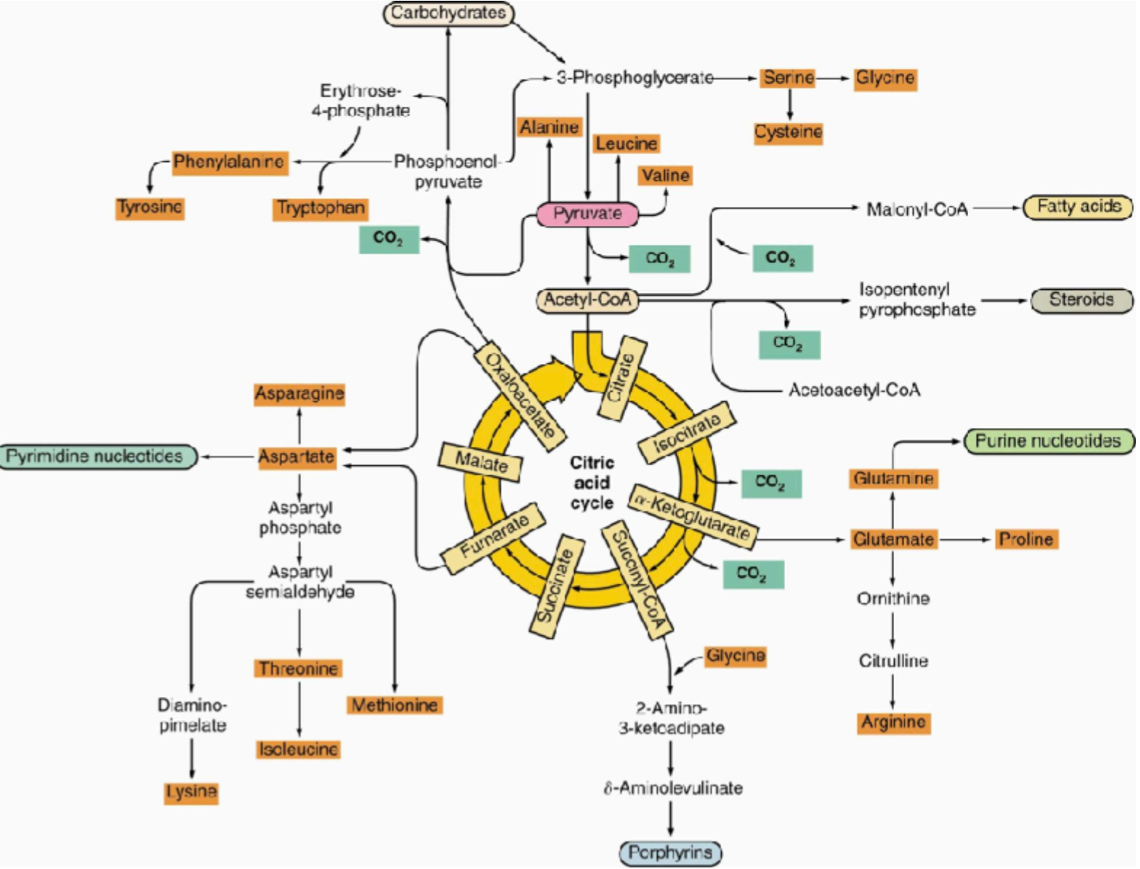
\includegraphics[width=0.7\linewidth]{Overview}
	\caption{This image shows an overview of many of the products stemming from the citric Acid Cycle. This ranges from amino acids, to nucleic acids, porphyrines, and more.}
	\label{fig:overview}
\end{figure}


\subsection{The actual synthesis of Amino Acids}

Amino acids are produced from intermediates of glycolysis of the TCA cycle or of the pentose phosphate patway. Nitrogen is transaminated onto these substrates from glutamine or glutamate

\begin{figure}
	\centering
	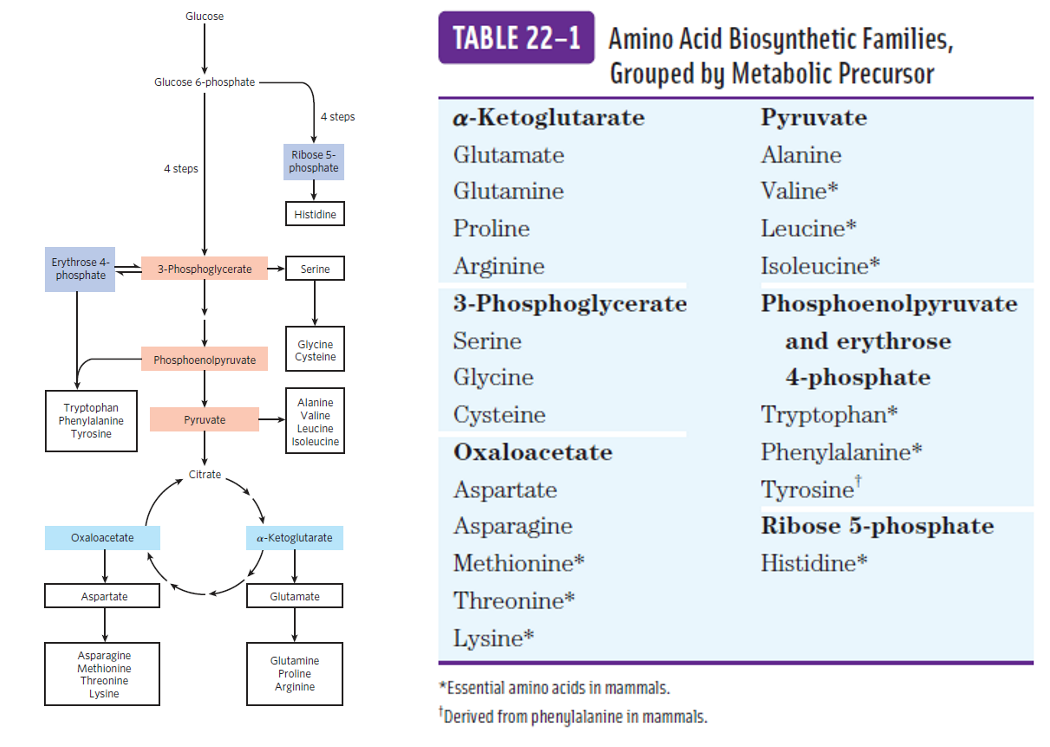
\includegraphics[width=0.7\linewidth]{amino_overview}
	\caption{the image on the left shows in which part of glycolysis we derive the amino-acids from. The table on the right shows the precursor for each amino acid.}
	\label{fig:aminooverview}
\end{figure}



\subsubsection{Prelude: Incorporating Nitrogon - Glutamate and Glutamine}

Nitrogen is required in amino acids. However, we humans can't get it from the atmosphere. That means we rely bacteria and archea to fix N2 from the atmosphere to produce ammonia. That ammonia then enters the cell metabolism and is incorporated into \textbf{\gls{Glutamate}} and \textbf{\gls{Glutamine}}.

\begin{figure}[H]
	\centering
	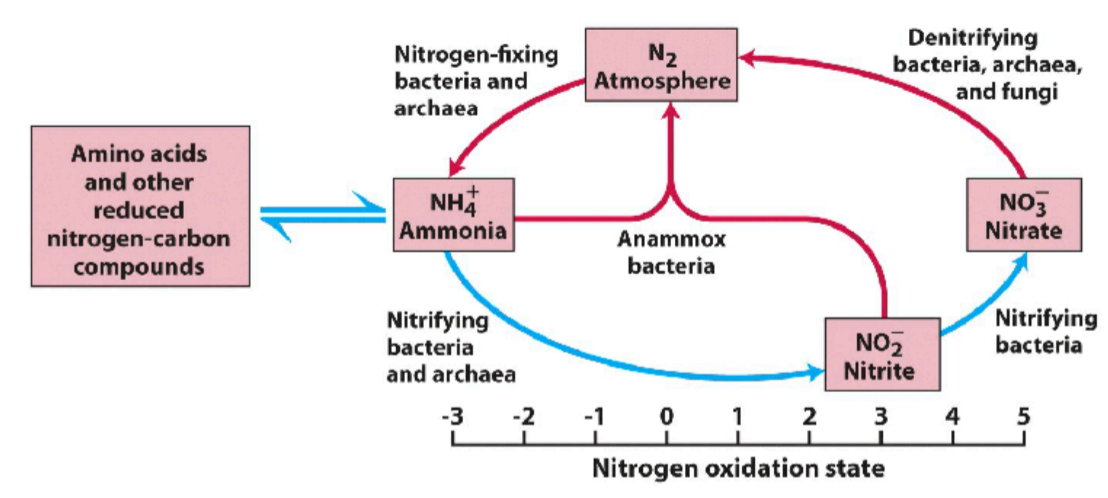
\includegraphics[width=0.4\linewidth]{nit_cyc}
	\caption{Shows the nitrogen cycle, which happens in bacteria and archea. Humans can absorb ammonia.}
	\label{fig:nitcyc}
\end{figure}

The production of glutamate in bacteria follows the production of glutamine. Here's what that looks like:
\begin{enumerate}
	\item Glutamine production (both in humans and bacteria): Glutamate + NH4+ $\rightharpoonup$ glutamine, through the enzyme \textbf{\gls{Glutamine synthase}} using a 1 ATP.
	\item Glutamate production (in bacteria): $\alpha$-ketoglutarate + glutamine $\rightharpoonup$ 2 glutamate, through the enzyme \textbf{\gls{Glutamate synthase}} using both an NAPDH and an ATP. This reaction is a \textbf{transamination} and how bacteria produce more glutamate.
\end{enumerate}

\begin{figure}[H]
	\centering
	\subfigure[Synthesis of Glutamate in bacteria using the enzyme glutamate synthase]{
		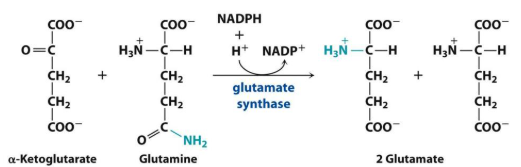
\includegraphics[width=0.5\textwidth]{mate_mech}
	}
	\hfill
	\subfigure[Synthesis of Glutamine in bacteria or humans using the enzyme glutamine synthase]{
		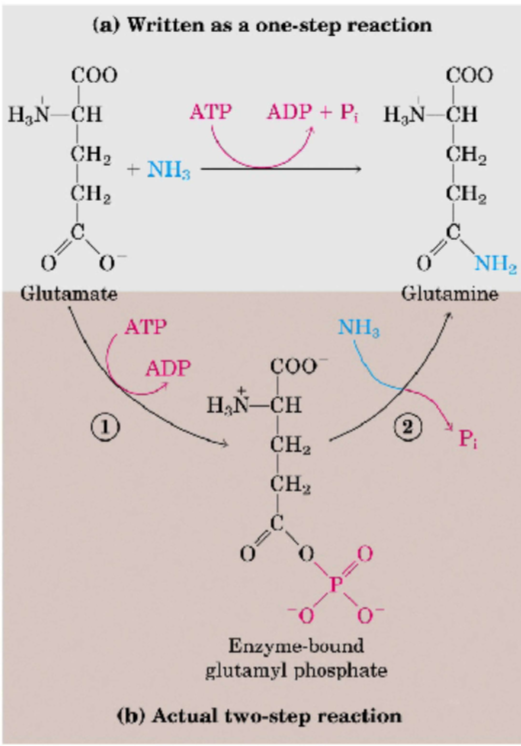
\includegraphics[width=0.3\textwidth]{amine_path}
	}
	\caption{Shows the synthesis of both glutamine and glutamate}
\end{figure}

Glutamate and glutamine are then used to transfer NH3 to a variety of different product, producing aminated molecules; these are called \textbf{\gls{transamination}} reactions. \\

\textbf{\gls{Glutamine amidotransferase}} is a common enzyme for transaminating glutamine. How the transamination happens:
\begin{enumerate}
	\item This enzyme is constituted by two domains, one that binds glutamine, the other binds the acceptor substrate.
	\item A Cys residue in the Glutamine-binding domain breaks the acidic bond and forms a glutamyl-enzyme intermediate
	\item NH3 travels to the NH3-acceptor domain
	\item There an activated substrate (usually activated by ATP) is aminated and released.
\end{enumerate}
\begin{figure}[H]
	\centering
	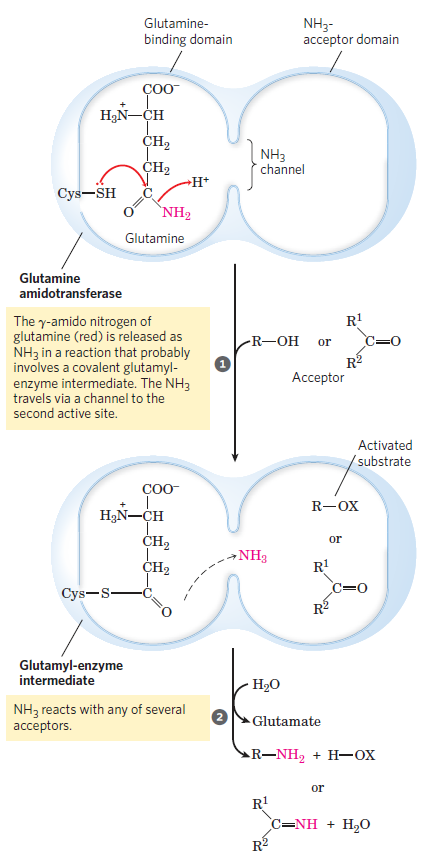
\includegraphics[width=0.5\linewidth]{nit_enz}
	\caption{The enzyme glutamine amidotransferase's mechanism.}
	\label{fig:nitenz}
\end{figure}


\subsubsection{Proline and Arginine}

\textbf{\gls{Proline}} is a cyclic derivative of glutamate. Here is its synthesis:
\begin{enumerate}
	\item Glutamate is phosphorylated
	\item Glutamyl-P is dephosphorylated and reduced
	\item Glutamate semialdehyde undergoes spontaneous cyclisation.
	\item Pyrroline-5-carboxylate is reduced to Proline.
\end{enumerate}

\textbf{\gls{Arginine}} is synthesized in a similar pathway:
\begin{enumerate}
	\item Glutamate is first acylated.
	\item $[Proline-equiv.]$ Acetylglutamate is phosphorylated.
	\item $[Proline-equiv.]$ Acetylglutamate-P is then reduced.
	\item The acylation impedes the cyclisation. Instead through further transamination and de-acylation Ornithine is produced.
	\item Ornithine is then converted to Arginine in the urea cycle (seen in lecture on Lipid biosynthesis).
\end{enumerate}

\begin{figure}[H]
	\centering
	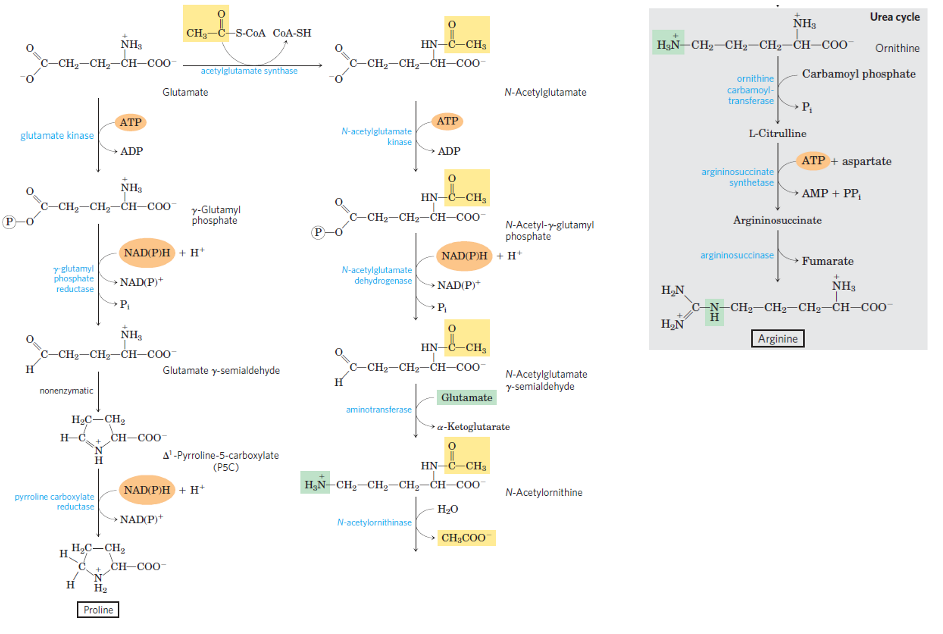
\includegraphics[width=0.6\linewidth]{pro_arg}
	\caption{Shows the pathway for the production of both Proline and Arginine, stemming from glutamate.}
	\label{fig:proarg}
\end{figure}


\subsubsection{Serine, Glycine, and Cysteine}

\textbf{\gls{Serine}} is formed from an intermediate of glycolysis: 3-phosphoglycerate. Cysteine and Glycine on the other hand are derivatives of Serine. \\

First the synthesis of Serine:
\begin{enumerate}
	\item Oxidation of 3-phosphoglycerate
	\item Transamination of 3-phosphooxypyruvate
	\item Dephosphorylation of 3-phosphoserine
\end{enumerate}

To continue to \textbf{\gls{Glycine}}, the enzyme \textbf{\gls{serine hydroxymethyltransferase}} removes a carbon atom from glycine. For this it uses tetrahydrofolate, as well as \gls{PLP} (activated vitamin B6) as a cofactor.
\begin{figure}[H]
	\centering
	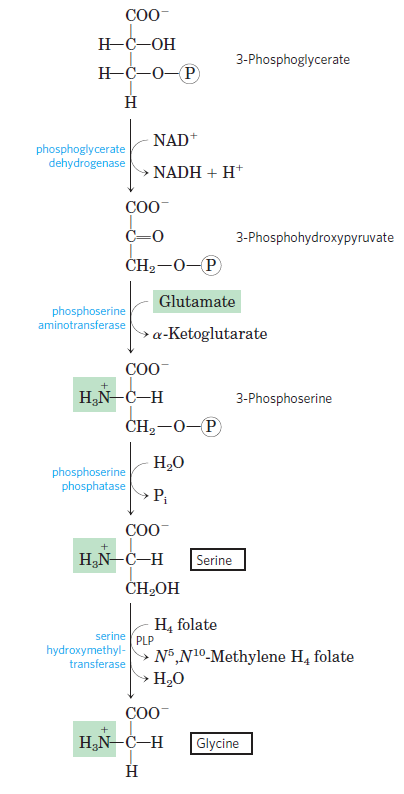
\includegraphics[width=0.3\linewidth]{ser_gly}
	\caption{The synthesis of Glycine and Serine. Glycine is a derivate of Serine.}
	\label{fig:sergly}
\end{figure}

In mammals \textbf{\gls{Cysteine}} is formed from \textbf{\gls{Serine}} and \textbf{\gls{Methionine}}. Here's how:
\begin{enumerate}
	\item Through a series of reactions Methionine becomes homocysteine.
	\item Homocysteine is condensed to bond with Serine to form cystathionine.
	\item Cystathionine is hydrolysed with a loss of NH4+ to form cysteine and \textbf{\gls{alpha-ketobutyrate}}.
\end{enumerate}

\begin{figure}[H]
	\centering
	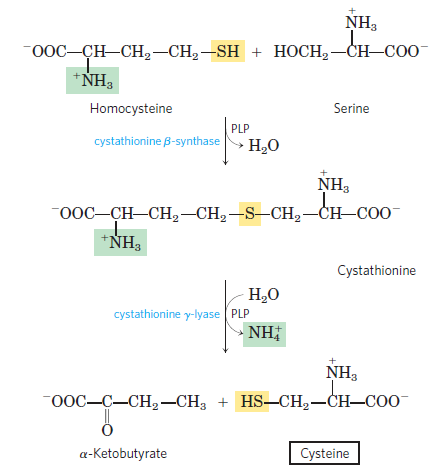
\includegraphics[width=0.3\linewidth]{cys}
	\caption{The snythesis of Cysteine from Serine and Methionine.}
	\label{fig:cys}
\end{figure}


\subsubsection{Aspartate, Aspargine, and Alanine}

Aspargine and Alanine are produced mainly in the liver. So, if you have too high concentrations of the two, something is probably off in your liver. \\

\textbf{\gls{Aspartate}}, \textbf{\gls{Asparagine}}, and \textbf{\gls{Alanine}} are produced the following way:
\begin{itemize}
	\item Aspartate: Transamination of oxaloacetate, catalyzed by \textbf{\gls{Aspartate transaminase (AST)}}.
	\item Asparagine: Amidation of aspartate by glutamine, catalyzed by \textbf{\gls{Asparagine Synthase}} using an ATP into AMP.
	\item Alanine: Transamination of pyruvate, catalyzed by \textbf{\gls{Alanine transaminase (ALT)}}.
\end{itemize}

\begin{figure}[H]
	\centering
	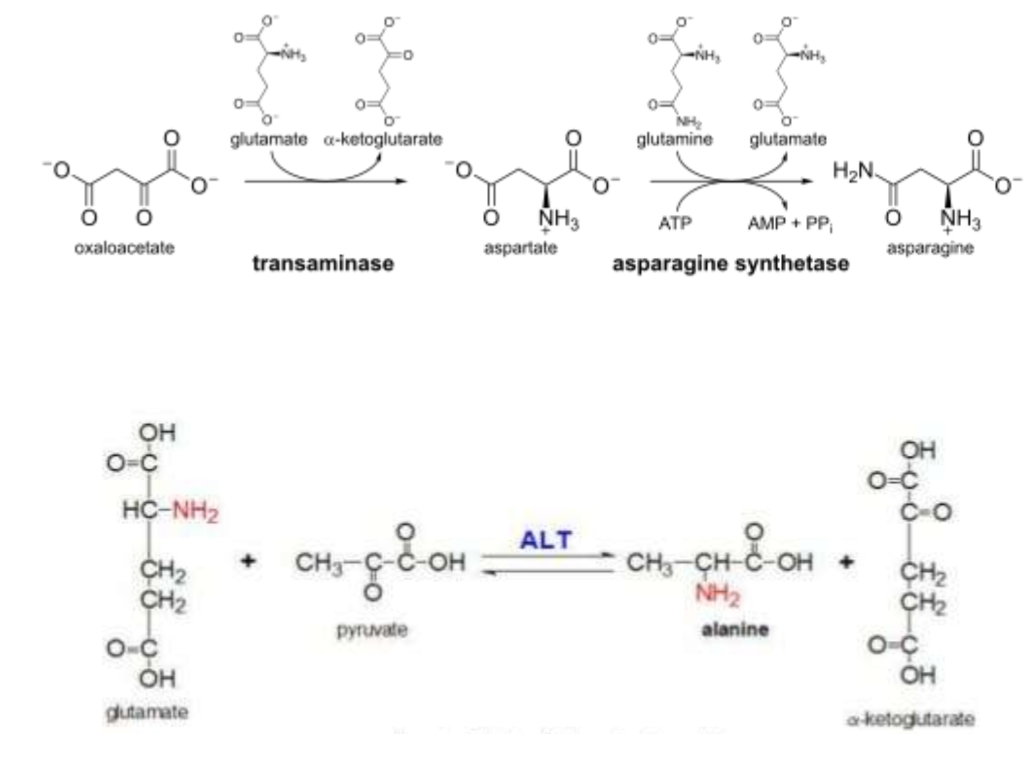
\includegraphics[width=0.7\linewidth]{asp_arg_ala}
	\caption{The synthesis of Aspartate (to become Aspartic Acid), Aspargine, and Alanine.}
	\label{fig:aspargala}
\end{figure}


\subsubsection{Essential Amino Acids}

Now, that leaves us with the \textbf{\gls{essential amino acids}}, which are those amino acids the human body can't synthesize. Instead we consume food to get to them. This even though they will often have precursors which would be in our body. Here is a quick overview:

\begin{figure}[H]
	\centering
	\subfigure[Essential amino acids with the precursors Oxaloacetate or pyruvate.]{
		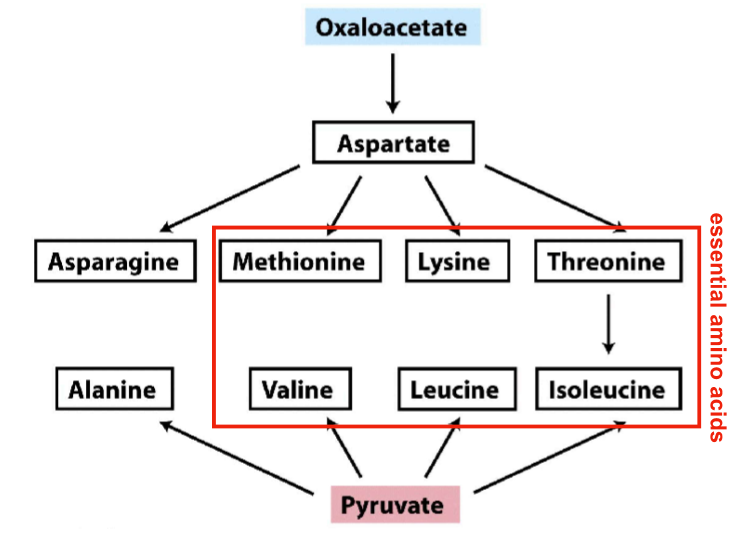
\includegraphics[width=0.4\textwidth]{ess_1}
	}
	\hfill
	\subfigure[Essential amino acids with the precursors Ribose 5-phosphate, Phosphoenolpyruvate and erythrose 4-phosphate.]{
		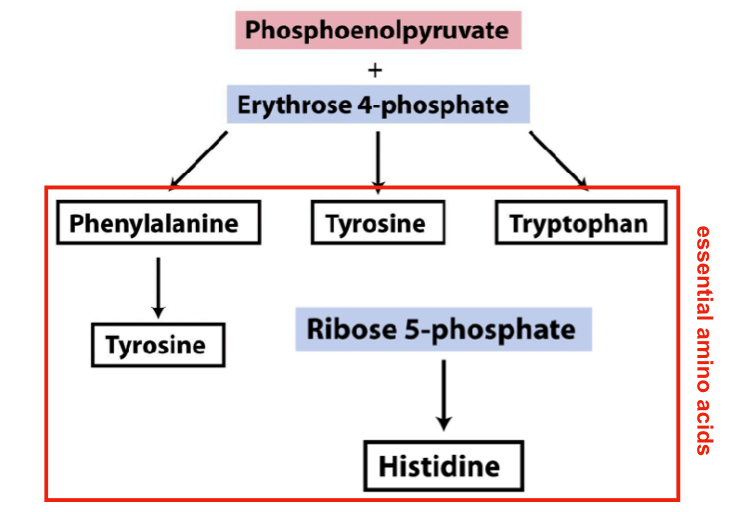
\includegraphics[width=0.45\textwidth]{ess_2}
	}
	\caption{}
\end{figure}

\subsection{Amino Acids derived Biomolecules}

Amino acids are not only the precursors for proteins. They are also precursors for lipid production, neurotransmitters, porphyrins, and hormones. 

\begin{figure}[H]
	\centering
	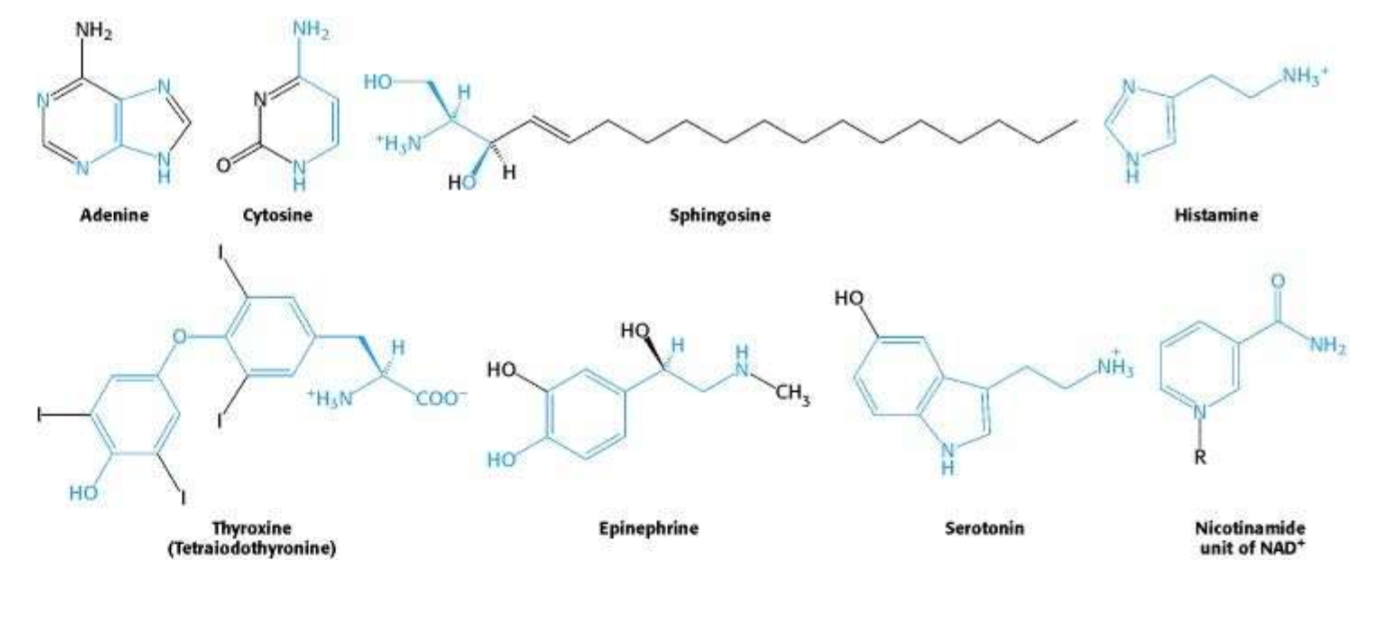
\includegraphics[width=0.5\linewidth]{aa_derivates_ex}
	\caption{Some examples of amino acids being precursors for other biomolecules.}
	\label{fig:aaderivatesex}
\end{figure}


\subsubsection{Porphyrins}

\textbf{\gls{Porphyrins}} are a group of herterocyclic compounds, that absorb strongly in the visible region of the EM spectrum. Metal complexes derived from porphyrins occur naturally. One very prominent example of a porphyrin is heme, which makes blood cells red, and is a cofactor of hemoglobin.

Glycine is the main precursor for the synthesis of porphyrins. Glutamate is an alternative sourcce. Here's how:
\begin{itemize}
	\item Glycine (mammals) reacts with succinyl-CoA to form $\alpha$-amino-ketodipate. This is then decarboxylated to \textbf{\gls{d-aminolevulinate}}.
	\item Glutamate (plants and bacteria): Through the reduction of Glutaminyl-tRNA, followed by the isomerization of glutamate semialdehyde, we also end up with d-aminolevulinate.
\end{itemize}

\begin{figure}[H]
	\centering
	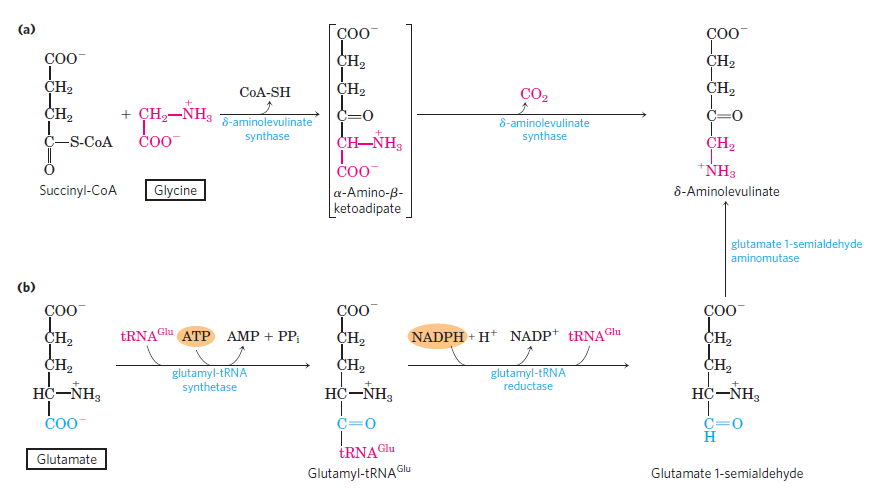
\includegraphics[width=0.5\linewidth]{por_glyglu}
	\caption{The biosynthesis of delta-aminolevuliante. mammals use glycine, while plants use glutamate.}
	\label{fig:porglyglu}
\end{figure}

\begin{figure}[H]
	\centering
	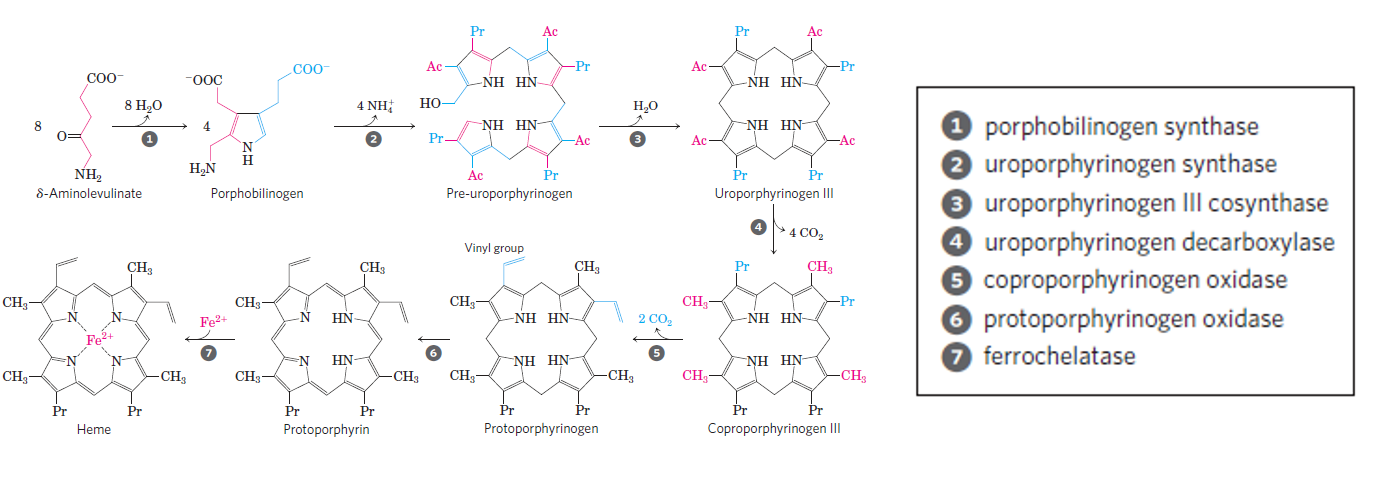
\includegraphics[width=0.7\linewidth]{por_synth}
	\caption{Biosynthesis of heme from delta-aminolevulinate.}
	\label{fig:porsynth}
\end{figure}

\begin{RemarkWithTitel}{Porphyria}
	 \textbf{\gls{Porphyria}} is a group of diseases which stems from the intermediates of porphyrin build up, negatively affecting the skin or nervous system. This is due to defects in the genes encoding the enzymes of the pathway. The nervous system porphyrias are also called acute porphyria as the symptoms are rapid in onset and last a short time. Cutaneous porphyria includes the skin symptoms, e.g., through a sensitivity to sunlight, but usually don't include the nervous system.
\end{RemarkWithTitel}


\begin{figure}[H]
	\centering
	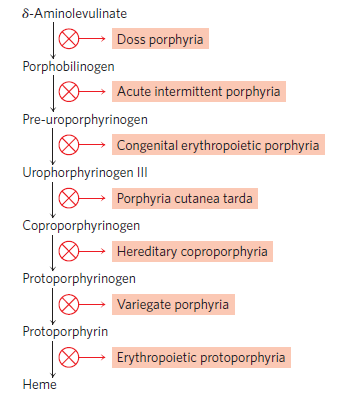
\includegraphics[width=0.3\linewidth]{por_sick}
	\caption{This image shows the types of diseases that stem from a certain enzyme defect. Accordingly the symptoms will vary, as the built up molecule will be different.}
	\label{fig:porsick}
\end{figure}

\begin{RemarkWithTitel}{Degradation and excretion of heme}
	\textbf{\gls{Heme}} from senescent erythrocytes are the origin for degraded hemes. It can also be degraded coming from other cell types. Senescent erythrocytes are degraded in the spleen. 
	\begin{enumerate}
		\item Here, Heme is first converted to \textbf{\gls{bilirubin}} in a two-step enzymatic process which employs biliverdin as an intermediate.
		\item These steps result in oxidation and opening of the heme ring. Bilirubin is then excreted into the plasma.
		\item Within hepatocytes, one or two molecules of glucuronic acid are attached to bilirubin, generating bilirubin momo/di-glucuronide. 
		\item These are excreted into bile canaliculi from where they are secreted in to the duodenum as part of bile.
	\end{enumerate} 
	
\end{RemarkWithTitel}


\subsubsection{Phosphocreatine}

\textbf{\gls{Phosphocreatine (Pcr)}}, a.k.a. creatine phosphate (CP a.k.a. Pcr) is a phosphorylated creatine molecule that serves as a rapidly mobilisable reserve of high-energy phosphates in skeletal muscle, myocard and the brain. This allows it to recycle ATP. 

\textbf{\gls{Creatine}}: the direct precursor of Phosphocreatine is produced from glycine and arginine with participation of Methionine as donor of a methyl group.

\begin{figure}[H]
	\centering
	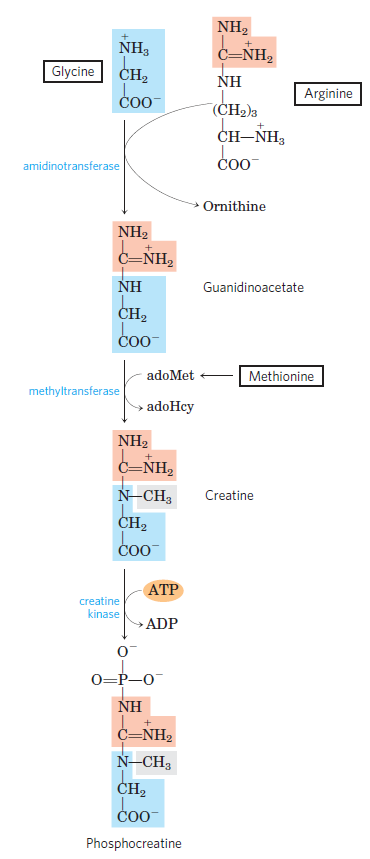
\includegraphics[width=0.3\linewidth]{creatine}
	\caption{Biosynthesis of Creatine and phosphocreatine.}
	\label{fig:creatine}
\end{figure}


\subsubsection{Glutathione}

\textbf{\gls{Glutahione}} is an antioxidant capable of preventing damage to cellular components caused by reactive oxygen species. It is a $\gamma$-peptide linkage between the carboxy group of glutamate side chain and cysteine. The carboxy group of cysteine is attached through a regular peptide bond to glycine. 

The GSH biosynthesis involves two ATP-dependent steps:
\begin{enumerate}
	\item \textbf{\gls{gamma-glutamylcysteine}} is synthesized from L-glutamate and cysteine, by the enzyme \textbf{\gls{glutamate-cysteine ligase (GCL)}}.
	\item glycine is added to the C-terminal of $\gamma$-glutamylcysteine. This condensation is catalyzed by \textbf{\gls{Glutathione synthetase}}.
\end{enumerate}

\begin{figure}[H]
	\centering
	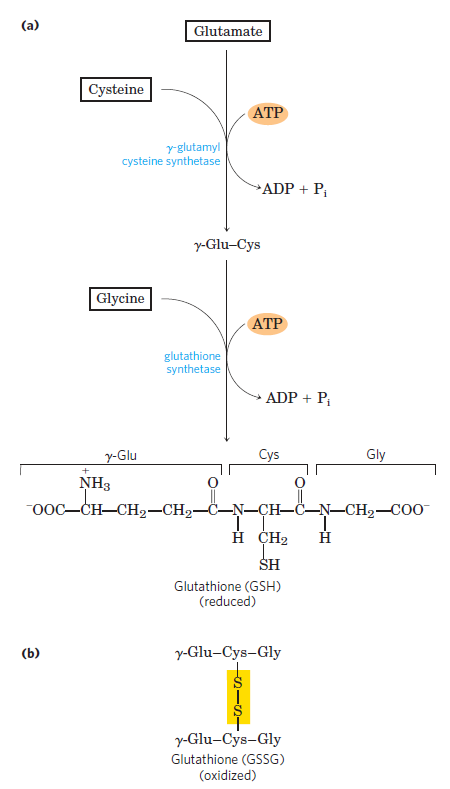
\includegraphics[width=0.3\linewidth]{gsh}
	\caption{The top picture shows the biosynthesis of GSH. The bottom picture shows the oxidized form of glutathione.}
	\label{fig:gsh}
\end{figure}

\subsubsection{Biogenic Amines}

\textbf{\gls{Biogenic amines}} are organic bases, which a low molecular weight, which are produced in many different cells (e.g., adrealine in adrenal modulla or histamine in mast cells and liver). Many biogenic amines are \textbf{\gls{neurotransmitter}} (e.g., acetylcholine, serotonin, histamine, epinephrine, and dopamine). They can also be agonists or dedicated receptors. \\

Biogenic amines are produced by modification (mostly decarboxylations and hydroxylations) of different amino acids:

\begin{figure}[H]
	\centering
	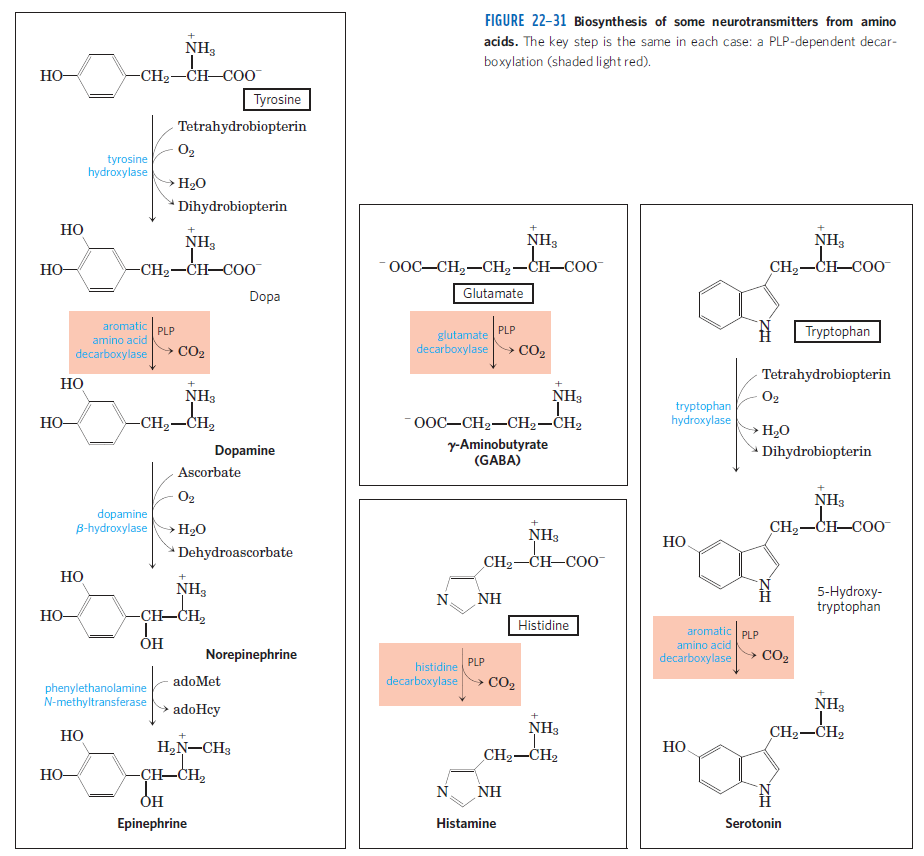
\includegraphics[width=0.5\linewidth]{biogenics}
	\caption{Biosynthesis of some neurotransmitters from amino acids.}
	\label{fig:biogenics}
\end{figure}


\subsubsection{Polyamines}

The biosynthesis of \textbf{\gls{Polyamines}} is highly regulated, nevertheless the function of polyamines is only partly understood. In their cationic ammonioum form, they bind to DNA and are compounds that are found at regularly spaced intervals. They have also been found to act as promoters of programmed ribosomal frameshifting in translation. \\

Spermidine and spermine are synthesized starting from ornithine. Ornithine itself is obtained from arginine in the urea cycle. 
\begin{itemize}
	\item Spermidine synthesis: from putrescine, using an aminoporpyl group from a decarboxylated S-adenosyl-L-methionine (SAM), which is catalyzed by spermidine synthase.
	\item Spermine synthesis: from the reaction of spermidine with SAM, which is catalyzed by spermine synthase.
\end{itemize} 


\section{Nucleic Acids in Biosynthesis}

\subsection{Biosynthesis of Nucleic Acids}

\textbf{\gls{Nucleotides}} are molecules consisting of a nucleoside and a phosphate group. They are precursors for:
\begin{itemize}
	\item \textbf{\gls{DNA}} and \textbf{\gls{RNA}}
	\item energy molecules such as \textbf{\gls{ATP}}, \textbf{\gls{GTP}}, \textbf{\gls{CTP}}, and \textbf{\gls{uridine triphosphate (UTP)}} 
	\item second messengers such as \textbf{\gls{cAMP}} and \textbf{\gls{cGMP}}
	\item key enzyme cofacators such as \textbf{\gls{CoA}}, \textbf{\gls{FAD}}, \textbf{\gls{NAD+}}, and \textbf{\gls{NADP+}}
\end{itemize}

Nucleotides contain either a \textbf{purine} or a \textbf{pyrimidine} base.  

\subsubsection{Biosynthesis of Purines}

\textbf{\gls{Purine}} is a heterocyclic aromatic compound that consists of a pyrimidine and fused to an imidazole ring.

The pathway of Purine production:
\begin{enumerate}
	\item It starts with the formation of 5-Phosphoribosyl pyrophosphate (PRPP) from 5-phosphoribose, which is formed in the pentose phosphate pathway.
	\item PRPP's pyrophosphate is displaced by an amide from a glutamine.
	\item Next, a glycine is incorporated.
	\item A carbon unit from folic acid coenzyme $N_{10}$-formyl-THF is added.
	\item A second amide is transferred from a glutamine to the first carbon of the glycine unit.
	\item The ring is closed.
	\item Carboxylation of the second carbon of the glycine unit is concomitantly added. This new carbon is modified by the addition of a third amide.
	\item Finally a second carbon unit from formyl-THF is added to the nitrogen group and the ring covalently closed to form the common purine precursor \textbf{\gls{inosine monophosphate (IMP)}}.
\end{enumerate} 

\begin{figure}[H]
	\centering
	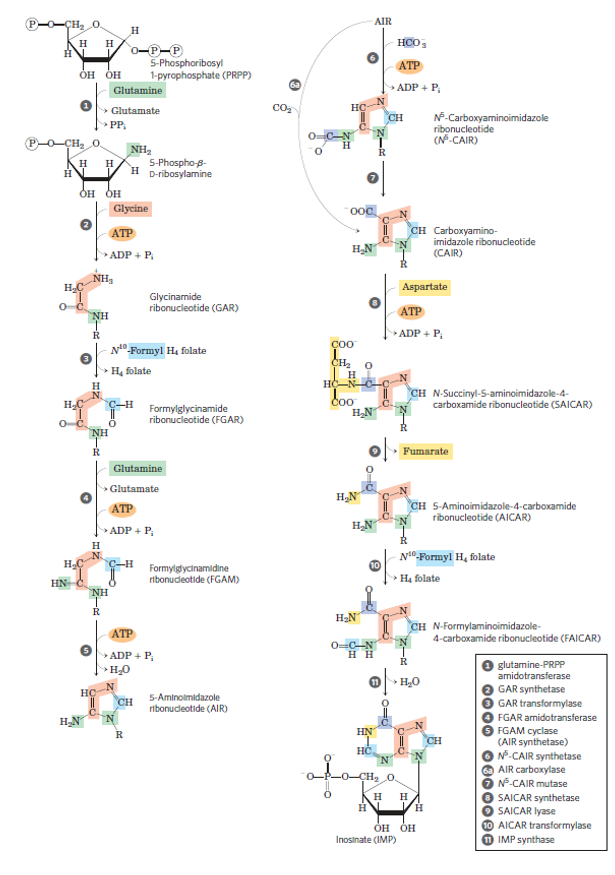
\includegraphics[width=0.6\linewidth]{puri_path1}
	\caption{De novo synthesis of purine nucleotides: construction of the purine ring of IMP. On the bottom right one can see all the involved enzymes.}
	\label{fig:puripath1}
\end{figure}

Creating the individual nucleic acids:

\begin{itemize}
	\item IMP is converted to \textbf{\gls{adenosine monophosphate (AMP)}} in two steps:
	\begin{enumerate}
		\item GTP hydrolysis fuels the addition of Aspartate to IMP, through the substitution of a carbonyl oxyxgen for a nitrogen forming the intermediate adenylosuccinate by adenylosuccinate synthase.
		\item Fumarate is then cleaved off forming AMP, caralyzed by \textbf{\gls{adenylosuccinate lyase}[adenylosuccinate lyase]}.
	\end{enumerate}
	\item IMP is converted to\textbf{\gls{guanosine monophosphate}} by:
	\begin{enumerate}
		\item the oxidation of IMP forming xanthylate. NAD+ is the electron acceptor.
		\item An amino group is inserted at the $C_{2}$, which is fuelled by ATP hydrolysis.+
	\end{enumerate}
\end{itemize}

\begin{figure}[H]
	\centering
	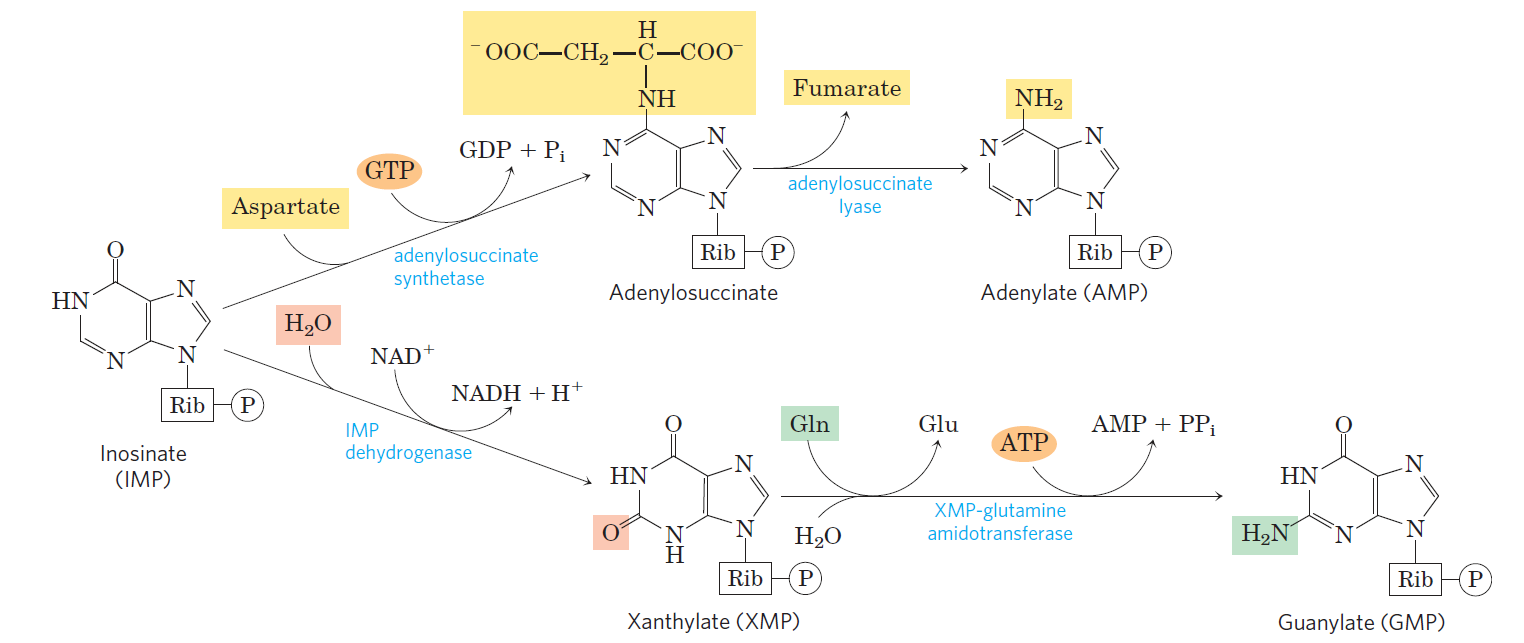
\includegraphics[width=0.8\linewidth]{puri_path2}
	\caption{Biosynthesis of AMP and GMP from IMP.}
	\label{fig:puripath2}
\end{figure}


\subsubsection{Biosynthesis of Pyrimidines}

\textbf{\gls{Pyrimidine}} is an aromatic heterocyclic organic compound.

Here is the pathway:
\begin{enumerate}
	\item It starts with the formation of \textbf{\gls{carbamoyl phosphate}} from glutamine and $CO_{2}$.
	\item \textbf{\gls{Aspartate carbamoyltransferase}} catalyzes a condensation reaction between aspartate and carbamoyl phosphate to form \textbf{\gls{carbamoyl aspartic acid}}.
	\item This is cyclized into \textbf{\gls{4,5-dihydroototic acid}} by \textbf{\gls{dihydroorotase}}. 
	\item which is then converted to orotate by \textbf{\gls{dihydroorotate oxidase}}.
	\item Orotate is covalently linked with a phosphorylated ribosyl unit.
	\item Orotidylate is decarboxylated to form \textbf{\gls{uridine monophosphate (UMP)}}.
	\item UMP is phosphorylated by two \textbf{\gls{kinases}} to form\textbf{\gls{uridine triphosphate (UTP)}} via two sequential reactions with ATP.
	\item \textbf{\gls{CTP}} subsequently formed by the amination of UTP by the\textbf{\gls{CTP synthetase}}, where glutamine is the NH3 donor and is fueled by ATP hydrolysis.
\end{enumerate}

\begin{figure}[H]
	\centering
	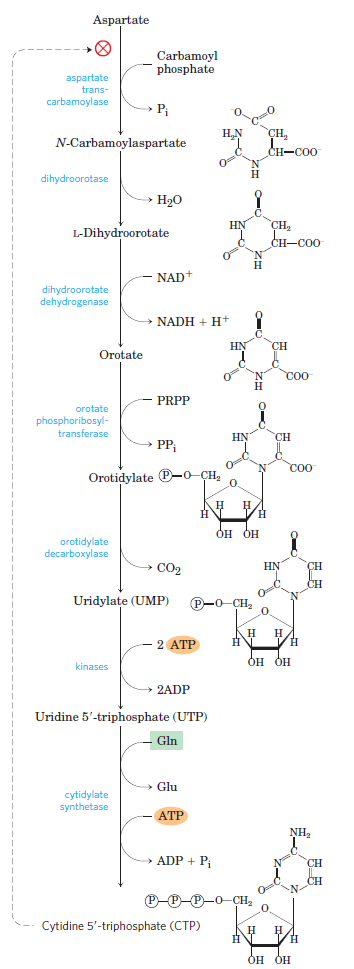
\includegraphics[width=0.3\linewidth]{pyri_path}
	\caption{De novo synthesis of pyrimidine nucelotides. Biosynthesis of UTP and CTP from orotidylate.}
	\label{fig:pyripath}
\end{figure}


\subsubsection{Reduction from Ribonucleotides to Deoxyribonucleotides}

The formation of ribonucleotides to deoxyribonucleotides is done through the removal of the 2'-hydroxyl group on the ribose ring of the nucleoside diphosphate. The enzyme \textbf{\gls{ribonucleotide reductase (RNR)}}.


\begin{figure}[H]
	\centering
	\subfigure[Structure of riboneuleotide reductase (RNR).]{
		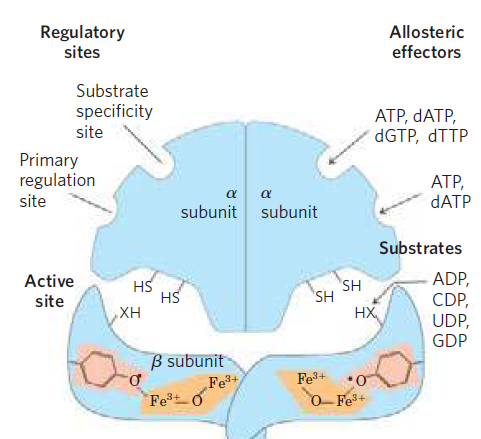
\includegraphics[width=0.35\linewidth]{rnr}
		\label{fig:rnr}
	}
	\hfill
	\subfigure[The mechansim for riboneucleotide reductase, turning ribonucleotides into deoxyribonucleotides.]{
		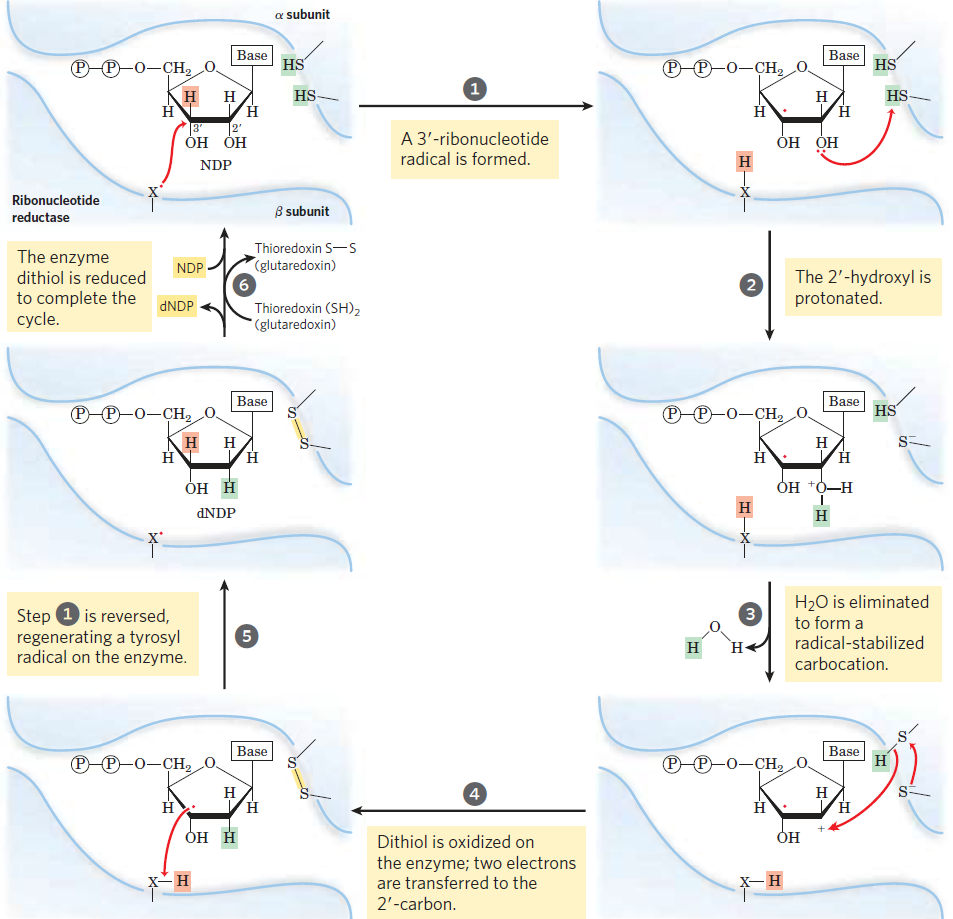
\includegraphics[width=0.5\linewidth]{deoxy_path}
		\label{fig:deoxypath}
	}
	\caption{The structure and mechanism of RNR.}
\end{figure}

\begin{RemarkWithTitel}{Regeneration of Ribonucleotide reductase (RNR)}
	In order for RNR to catalyze the next reduction it has to be regenerated. This means the disulfide bond has to broken into to sulfide groups. For this we have an electron chain which has two possible pathways:
	\begin{enumerate}
		\item NAPDH
		\item GSSG (oxidized state)
		\item Glutaredoxin
		\item RNR
	\end{enumerate}
	Or:
	\begin{enumerate}
		\item NAPDH
		\item FAD (oxidized state)
		\item Thioredoxin
		\item RNR
	\end{enumerate}
	
	\begin{figure}[H]
		\centering
		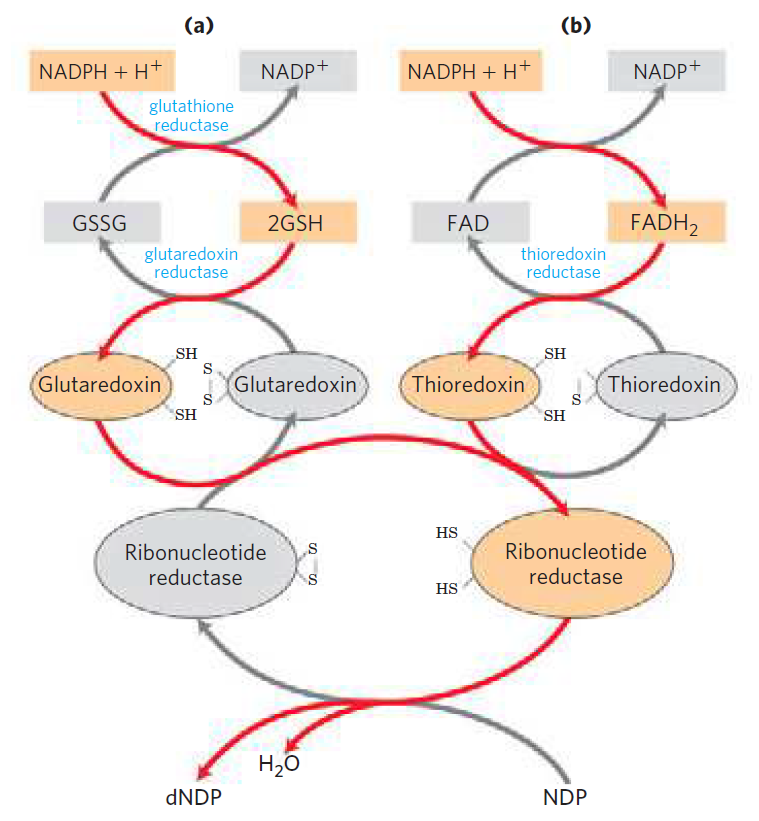
\includegraphics[width=0.5\linewidth]{rnr_regen}
		\caption{Shows the regeneration of RNR. Red arrows indicate electron movement, orange molecules are the reduced molecule, grey the oxidized. At the very bottom is the reduction of ribonucleotides to deoxyribonucleotides.}
		\label{fig:rnrregen}
	\end{figure}
	
\end{RemarkWithTitel}


\subsubsection{Biosynthesis of Thymidylate}

\textbf{\gls{Thymidylate (dTMP)}} is a component of DNA. It is synthesized de novo from deoxyuridylate (dUMP) and methylenetetrahydrofolate by \textbf{\gls{tyms}.} Dihydrofolate is a by-product. \\

dTMP is produced in the nuclear lamina, which is where DNA replication happens. DNA can't tell the difference betwee dUMP and dTMP. So, if there is a lack of dTMP uracil can be misintegrated into the DNA leading to point mutations if not repaired properly.

\begin{RemarkWithTitel}{Consequences of dTMP lacking} The lack of dTMP can have some consequences, due to the DNA being messed up: 
	\begin{itemize}
		\item Can cause neural tube defects, megalobastic anemia, and immune system problems.
		\item Pregnant women are more likely to have a \textbf{\gls{folate}} deficiency, which is why it is often supplemented.
		\item Drugs that block \textbf{TYMS} or \textbf{\gls{dihydrofolate_reductase}} (DHFR, the folate regenerator) slow down cell division and are used to treat cancer.
	\end{itemize} 
\end{RemarkWithTitel}
 
\begin{figure}[H]
	\centering
	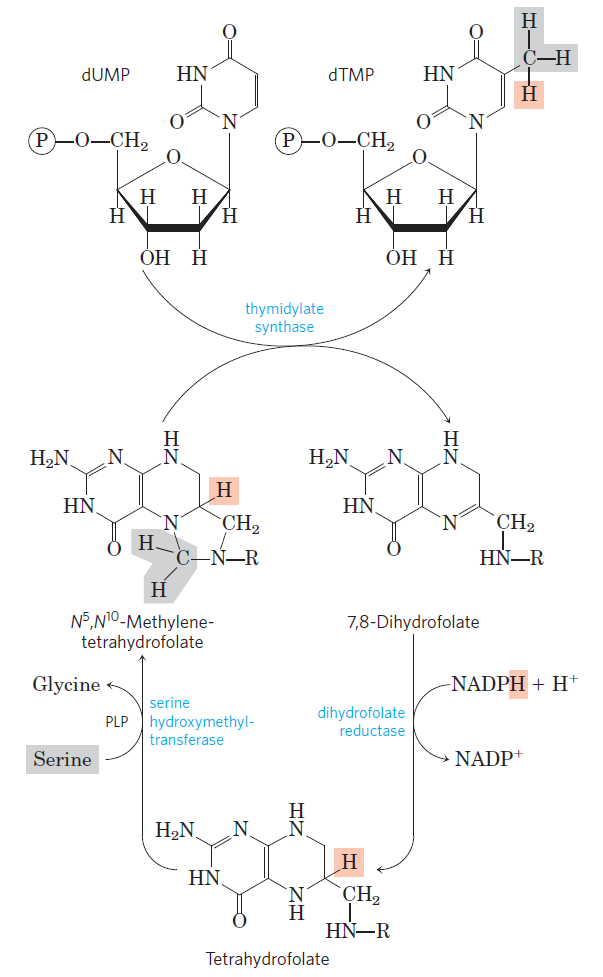
\includegraphics[width=0.4\linewidth]{dTMP_path}
	\caption{The conversion of dUMP to dTMP by TYMS and DHFR.}
	\label{fig:dtmppath}
\end{figure}


\subsection{Disposal of Nucleic Acids}
\subsubsection{Purines Disposal}

Purines are degraded to \textbf{\gls{uric acid}}, here's how:
\begin{enumerate}
	\item Phosphate is hydrolyzed by \textbf{\gls{5'-nucleotidase}}.
	\item \textbf{\gls{Adenosine}} is deaminated to \textbf{\gls{inosine}}.
	\item Inosine loses the ribose to form \textbf{\gls{hypoxanthine}}
	\item Through two oxidative reactions that is converted to uric acid.
\end{enumerate}

\begin{figure}[H]
	\centering
	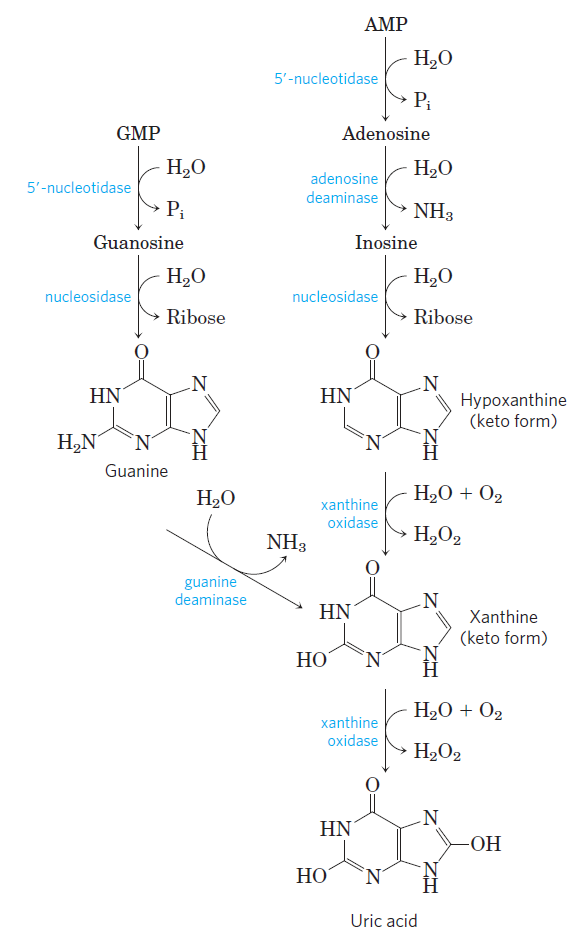
\includegraphics[width=0.4\linewidth]{ump_deg}
	\caption{Catabolsim of purine nucleotides.}
	\label{fig:umpdeg}
\end{figure}


\begin{RemarkWithTitel}{Degradation Purine}
	GMP follows a similar pathway, just that it has one deamination less in its degraditive pathway.
\end{RemarkWithTitel}


\subsubsection{Pyrimidines Disposal}

Pyrimidines are ultimately catabolized to $CO_{2} and H_{2}O$, and \textbf{urea}. 

Let's start with Cytosine:
\begin{enumerate}
	\item Cytosine gets broken down into Uracil.
	\item Uracil gets further broken down N-carbamoyl-$\beta$-alanine.
	\item That gets broken down to $\beta$-\gls{Alanine}, by \textbf{\gls{beta-ureidopropionase}}, with CO2 and ammonia as by-products
\end{enumerate}

Thymine's catabolism:
\begin{enumerate}
	\item Thymine is broken down into \textbf{\gls{beta-aminoisobutyrate}}.
	\item This is further broken down into \textbf{\gls{methylmalonyl semialdehyde}}(intermediate of valine catabolism).
	\item Which is then converted into \textbf{\gls{succinyl-CoA}}, which then enters the citric acid cycle.
\end{enumerate}

\begin{figure}[H]
	\centering
	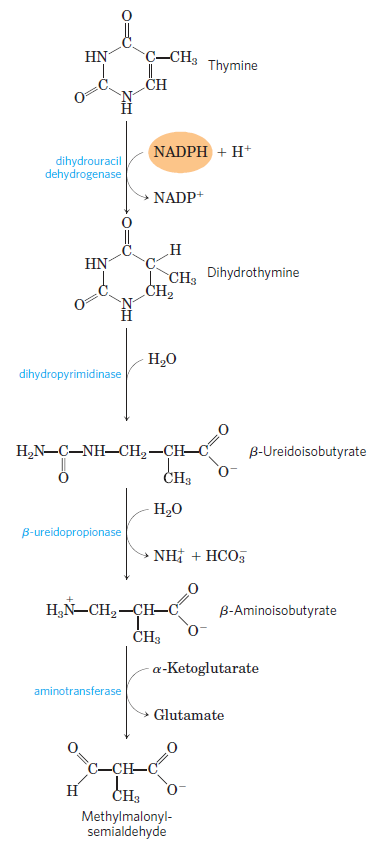
\includegraphics[width=0.3\linewidth]{pyr_dis}
	\caption{The catabolism of pyrimidines.}
	\label{fig:pyrdis}
\end{figure}


\begin{RemarkWithTitel}{Consequences of Genetic Defects: Severe combined immune deficiency}
	Genetic defects in the catabolism lead to diseases in humans. Defects in the enzyme adenosine deaminase leads to \textbf{\gls{severe combined immune deficiency (ADA-SCID)}}. Why immunodeficiency? Because the defect results in an accumulation of deoxyadenosine, which in turn leads to a buildup of dATP in all cells. This is turn inhibits ribonucleotide reductase, preventing DNA cells. This means cells can't divide. T and B cells, with there high mitotic rate are very susceptible to this condition.
\end{RemarkWithTitel}

\subsubsection{Salvage Pathways}

Instead of catabolising the nucleotides there are also \textbf{\gls{salvage pathways}} which recover bases and nucleosides that are formed in the degradation of RNA and DNA. 

For \textbf{Pyrimidines}:
\begin{itemize}
	\item \textbf{\gls{uridine monophosphate (UMP)}} regeneration:
	\begin{enumerate}
		\item \textbf{\gls{Uridine phosphorylase}} or \textbf{\gls{pyrimidine-nucleoside phosphorylase}} adds ribose 1-phosphate to the free base uracil forming \textbf{\gls{uridine}}.
		\item \textbf{\gls{Uridine-cytidine kinase}} can then phosphorylate this nucleoside into \textbf{UMP}.
	\end{enumerate}
	\item \textbf{TMP} regeneration:
	\begin{enumerate}
		\item \textbf{\gls{Thymidine phosphorylase}} or \textbf{\gls{pyrimidine-nucleoside phosphorylase}} adds 2-deoxy-$\alpha$-D-ribose 1-phosphate to thymine, forming \textbf{\gls{Thymidine}}.
		\item \textbf{\gls{Thymidine kinase}} can then phosphorylate this compound into \textbf{TMP}.
	\end{enumerate}
	\item \textbf{CMP} and \textbf{dCMP} regeneration has multiple options: 
	\begin{itemize}
			\item Salvage it along the uracil pathway, through \textbf{\gls{cytidine deaminase}}, which converts them \textbf{\gls{uridine}} and \textbf{\gls{deoxyuridine}}, respectively
			\item \textbf{\gls{Uridine-cytidine kinase}} can phosphorylate them into \textbf{CMP} or \textbf{dCMP}.
	\end{itemize}
\end{itemize}

For \textbf{Purines}: \textbf{\gls{Phosphoribosyltransferases}} add phosphoribosyl pyrophosphate to bases, creating the nucleoside monophosphate (\gls{adenosine monophosphate (AMP)}, GMP). There are two types of phosphoribosyltransferases:
\begin{enumerate}
	\item \textbf{\gls{adenine phosphoribosyltransferases (APRT)}},
	\item \textbf{\gls{hypoxanthine-guanine phosphoribosyltransferases (HGPRT)}}.
\end{enumerate}


\subsection{\gls{Chemotherapics} Targeting Nucleotide Metabolism}

Cancer cells usually  grow at faster rates than normal cells. As a consequence they have a higher need for nucleotides (for their DNA replication and RNA transcription), meaning they are more susceptible to the inhibition of nucleotide synthesis. For example some commonly used anti cancer drugs inhibit thymidylate synthesis.
\begin{figure}[H]
	\centering
	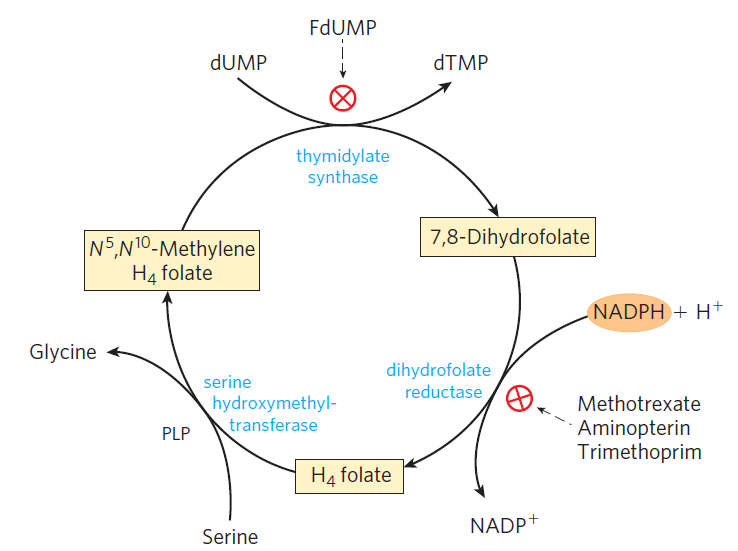
\includegraphics[width=0.4\linewidth]{cancer_inhib}
	\caption{Thymidylate synthesis and folate metabolism as targets of chemotherapy.}
	\label{fig:cancerinhib}
\end{figure}



\end{document}